% !TEX root = main.tex
% Main text: abstract through conclusion. Formal assumptions, full statements and proofs are in the appendix.
\begin{abstract}
A two-block Transformer can express both direct and step-by-step modular counting,
yet the two supervision formats can have different learning times.
From the same structured initialization and with the same trained parameters, outcome-supervised
cross-entropy flow has an exponentially long plateau at near-chance correct-answer probabilities, while process supervision learns
the recurring transition in polynomial time. The mechanism is a contraction coefficient $\lambda$:
unseen letters hide outcome credit on the scale $\lambda^n$, whereas displayed states expose a local
innovation controlled by $1-\lambda^2$. A Transformer score expansion connects this data structure
to gradient credit and training time. We also prove robustness to fixed query--key perturbations
and finite-accuracy full-prefix routing within a tied feature family. Experiments distinguish
prior fitting from rule learning and test routing and pretrained-model transfer. A reversal in
object tracking identifies a limit of the mechanism. The matched guarantee uses supplied routing
and small initialization; unrestricted feature and routing discovery remains open.
\end{abstract}

% ===================================================================
\section{Introduction}
\label{sec:intro}

A final-answer algorithm and a step-by-step algorithm can both fit inside one Transformer,
yet gradient training can reach them at very different speeds. We isolate this optimization
question using modular counting. Proposition~\ref{prop:represent} constructs exact executors
for both formats in the same two-block architecture. Intermediate supervision is known to
help reasoning \citep{nye2021scratchpads,wei2022cot,lightman2023verify}; here we trace its
benefit from the statistical information in a label to a learning-time separation.

\paragraph{Matched optimization separation.}
For the supplied-routing seed, fix the architecture, initialization and trained parameters
and change only the supervised objective. At executor head width $d_{\mathrm h}=\Theta(n)$
and initialization scale $\varepsilon=\Theta(n^{-1/2})$, with a sufficiently small fixed
constant, fixed $K,p\ne1/2$ and the alignment conditions of Theorem~\ref{thm:joint}(i), \cref{cor:matched-separation} gives
\[
 T_{\mathrm{out}}\ge c\lambda^{-n},\qquad
 T_{\mathrm{step}}=O(n^{5/2}\log n).
\]
The first time measures how long outcome flow remains near initialization with
near-chance correct-answer probabilities;
the second bounds when the recurring transition has persistent positive margins.
With the initial state, formatting and final-answer copy correctly established, those
transition margins generate the whole thought sequence by induction. Theorem~\ref{thm:joint}
focuses on the repeated transitions at $t\ge2$; the exact executors specify the boundary operations.

\paragraph{Mechanism and scope.}
Each unseen letter contracts a feature's final-count correlation by $\lambda<1$.
Small initialization makes terms that read few letters dominate the gradient; displaying
the previous state exposes a local innovation instead. The margin sum $R(t)$ removes the
state-only prior, and the minimum margin $M(t)$ records transition success
(\cref{eq:binary-rule-observables}). The matched result uses supplied routing, zero readout
and a small-initialization regime with MLP biases bounded away from zero after normalization.
The learned full-prefix result uses a different tied feature family and fixed unequal
mobilities, and guarantees finite accuracy. A two-path diagnostic with supplied
count averaging learns outcomes outside the fixed-pattern initialization regime
(\cref{app:two-path}); the tested seeds are not yet covered by the local trap's basin proof.
Empirical tests extend beyond these families.

\begin{figure}[t]
\centering
%% Figure 1 (pgfplots). Data: results/paper/zero_readout_n16_8k (seeds 42-51, median and 25th-75th percentile band),
%% results/paper/fig2/n8_s42.json (target A_r) and results/paper/exact_spectra/sigma_sweep/s42_sg0.02.txt (Jacobian J_r).
\definecolor{stepc}{HTML}{0072B2}\definecolor{outc}{HTML}{D55E00}\definecolor{theoc}{HTML}{009E73}
\definecolor{modelc}{HTML}{7B4F9E}\definecolor{mutedc}{HTML}{6E6E6E}
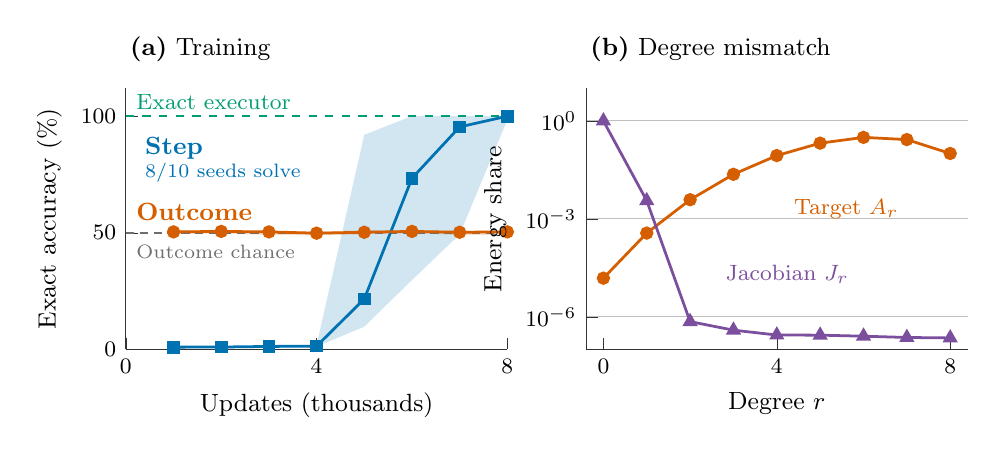
\begin{tikzpicture}
\pgfplotsset{every axis/.style={width=0.53\linewidth, height=4.9cm, axis line style={black!80}, tick style={black!80},
  tick label style={font=\footnotesize}, label style={font=\small}, title style={font=\small, at={(0,1)}, anchor=south west, xshift=-2pt}},
  every axis plot/.append style={line width=1pt}}
\begin{axis}[name=train, title={\textbf{(a)} Training}, xlabel={Updates (thousands)}, ylabel={Exact accuracy (\%)},
  xmin=0, xmax=8, ymin=0, ymax=112, xtick={0,4,8}, ytick={0,50,100}, axis x line*=bottom, axis y line*=left, clip=false]
  \addplot[draw=none, fill=stepc, fill opacity=0.18, forget plot] coordinates {(1,0.55) (2,0.73) (3,0.82) (4,1.25) (5,9.77) (6,29.75) (7,49.33) (8,98.40) (8,100.00) (7,100.00) (6,100.00) (5,92.03) (4,1.90) (3,1.40) (2,1.35) (1,1.35)};
  \addplot[draw=none, fill=outc, fill opacity=0.18, forget plot] coordinates {(1,49.52) (2,49.73) (3,49.05) (4,48.92) (5,49.35) (6,49.92) (7,48.97) (8,49.15) (8,50.70) (7,50.70) (6,51.20) (5,51.08) (4,50.60) (3,50.70) (2,51.08) (1,51.08)};
  \addplot[theoc, dashed, line width=0.9pt, domain=0:8, samples=2] {100};
  \addplot[mutedc, densely dashed, line width=0.8pt, domain=0:8, samples=2] {50};
  \addplot[stepc, mark=square*, mark size=1.8pt] coordinates {(1,1.00) (2,1.05) (3,1.30) (4,1.45) (5,21.65) (6,73.40) (7,95.40) (8,100.00)};
  \addplot[outc, mark=*, mark size=1.9pt] coordinates {(1,50.40) (2,50.60) (3,50.40) (4,49.85) (5,50.25) (6,50.60) (7,50.25) (8,50.40)};
  \node[anchor=south west, font=\footnotesize, text=theoc, inner sep=1pt] at (axis cs:0.15,101.5) {Exact executor};
  \node[anchor=west, font=\small\bfseries, text=stepc] at (axis cs:0.2,86) {Step};
  \node[anchor=west, font=\scriptsize, text=stepc] at (axis cs:0.2,76) {8/10 seeds solve};
  \node[anchor=south west, font=\small\bfseries, text=outc, inner sep=1pt] at (axis cs:0.15,54) {Outcome};
  \node[anchor=north west, font=\scriptsize, text=mutedc, inner sep=1pt] at (axis cs:0.15,46) {Outcome chance};
\end{axis}
\begin{semilogyaxis}[at={(train.east)}, anchor=west, xshift=1.0cm, title={\textbf{(b)} Degree mismatch}, xlabel={Degree $r$},
  ylabel={Energy share}, xmin=-0.4, xmax=8.4, ymin=1e-7, ymax=10, xtick={0,4,8}, ytick={1e-6,1e-3,1},
  ymajorgrids, major grid style={black!25}, axis x line*=bottom, axis y line*=left]
  \addplot[outc, mark=*, mark size=1.9pt] coordinates {(0,1.5259e-05) (1,3.6621e-04) (2,3.8452e-03) (3,2.3071e-02) (4,8.6517e-02) (5,2.0764e-01) (6,3.1146e-01) (7,2.6697e-01) (8,1.0011e-01)};
  \addplot[modelc, mark=triangle*, mark size=2.2pt] coordinates {(0,9.9641e-01) (1,3.5840e-03) (2,7.1281e-07) (3,3.9081e-07) (4,2.7680e-07) (5,2.7450e-07) (6,2.5510e-07) (7,2.3310e-07) (8,2.2560e-07)};
  \node[anchor=north, font=\footnotesize, text=outc] at (axis cs:5.6,8e-3) {Target $A_r$};
  \node[anchor=west, font=\footnotesize, text=modelc] at (axis cs:2.6,2e-5) {Jacobian $J_r$};
\end{semilogyaxis}
\end{tikzpicture}

\caption{\textbf{Same architecture and task, different training behavior.}
(a)~Counting with $n=16$, $K=2$ and zero readout: median exact continuation accuracy and interquartile band over ten paired seeds, $8$k
updates; the dashed line marks the exact executor that both formats admit (\cref{prop:represent}).
(b)~A separate $n=8$, $K=2$, $\initscale=0.02$ measurement with nonzero readout: target and Jacobian energy occupy different interaction degrees, defined by the number of letters a component depends on jointly (\cref{app:spectrum}).}
\label{fig:overview}
\end{figure}

\needspace{3\baselineskip}
\paragraph{Contributions.}
\begin{itemize}[leftmargin=*,itemsep=3pt,topsep=3pt]
\item \textbf{A matched learning-time separation.} Both supervision formats admit exact
solutions in one architecture, but the same supplied-routing seed yields exponential
outcome escape time and polynomial transition learning (\cref{prop:represent,cor:matched-separation}).
\item \textbf{A data-to-gradient mechanism.} Fourier contraction and a Transformer
score expansion quantify hidden outcome credit; displayed states retain local rule
credit (\cref{thm:main,thm:separation,thm:outcome-end}).
\item \textbf{Routing and empirical tests.} We prove fixed query--key robustness and
learned full-prefix routing, and measure prior fitting, rule learning and transfer
(\cref{thm:joint,sec:experiments}).
\end{itemize}

% ===================================================================
\section{Setup}
\label{sec:setup}
\label{sec:setting}

Modular counting keeps the state space fixed as the prompt grows. What increases is the number of updates hidden behind the
answer. We can therefore lengthen the computation without changing the prediction problem at its end.

\begin{definition}[Counting modulo $K$]
\label{def:task}
A prompt has a start count $s_0$, uniform on $\mathbb Z_K$, and letters $w_1,\ldots,w_n$ drawn i.i.d.\ from an alphabet
in which a fixed query letter $w^\star$ has probability $p\in(0,1)$. With $b_t=\mathbf 1[w_t=w^\star]$,
\begin{equation}
 s_t=s_{t-1}+b_t\pmod K,\qquad t=1,\ldots,n,
 \label{eq:tracking}
\end{equation}
and the answer is $y=s_n$.
\end{definition}

\begin{definition}[Contraction coefficient]
\label{def:lambda}
For counting modulo $K$,
\begin{equation}
 \mixrate=\max_{1\le j<K}\bigl|1-p+p\,e^{2\pi\mathrm ij/K}\bigr|=\bigl|1-p+p\,e^{2\pi\mathrm i/K}\bigr|.
 \label{eq:lambda}
\end{equation}
\end{definition}

\begin{figure}[t]
\centering
\resizebox{\linewidth}{!}{% Conceptual figure: counting modulo K as a cyclic chain, and what each supervision format sees.
\begin{tikzpicture}[>=Stealth, font=\small,
  state/.style={circle, draw=royalazure!80!black, fill=royalazure!12, minimum size=7mm, inner sep=0pt},
  tok/.style={rectangle, rounded corners=2pt, draw=black!45, fill=black!4, minimum width=7mm, minimum height=5.5mm, inner sep=1pt},
  sup/.style={rectangle, rounded corners=2pt, draw=royalazure!80!black, fill=royalazure!12, minimum width=7mm, minimum height=5.5mm, inner sep=1pt},
  hid/.style={rectangle, rounded corners=2pt, draw=black!30, dashed, fill=white, text=black!45, minimum width=7mm, minimum height=5.5mm, inner sep=1pt}]

% ---------------- (a) cyclic chain ----------------
\begin{scope}[shift={(0,0)}]
  \foreach \i/\lab in {0/0, 1/1, 2/2, 3/{K{-}1}} {
    \node[state] (c\i) at ({90-\i*90}:1.25) {$\lab$};
  }
  \foreach \i/\dir in {0/90, 1/0, 2/-90, 3/180} {
    \draw[->, black!55] (c\i) to[out=\dir+28, in=\dir-28, looseness=6] node[pos=0.5, font=\scriptsize, fill=white, inner sep=0.5pt] {$1{-}p$} (c\i);
  }
  \draw[->, thick, royalazure] (c0) to[bend left=22] node[font=\scriptsize, above right=-1pt] {$p$} (c1);
  \draw[->, thick, royalazure] (c1) to[bend left=22] node[font=\scriptsize, below right=-1pt] {$p$} (c2);
  \draw[->, thick, royalazure, dashed] (c2) to[bend left=22] node[font=\scriptsize, below left=-1pt] {$p$} (c3);
  \draw[->, thick, royalazure] (c3) to[bend left=22] node[font=\scriptsize, above left=-1pt] {$p$} (c0);
  \node[align=center, font=\footnotesize] at (0,-2.6)
    {$s_t=s_{t-1}+b_t\ (\mathrm{mod}\ K)$\\[2pt] $\mathbf T=(1-p)\,\mathbf I+p\,\mathbf R$};
  \node[font=\small\bfseries] at (-2.3,1.75) {(a)};
\end{scope}

% ---------------- (b) what each format supervises ----------------
\begin{scope}[shift={(3.4,0.95)}]
  \node[font=\small\bfseries] at (-0.35,0.8) {(b)};
  % outcome row
  \node[anchor=west, font=\footnotesize] at (0,0.8) {Outcome: supervise $s_n$ only};
  \node[tok] (o0) at (0.45,0) {$s_0$};
  \node[tok] (ow1) at (1.35,0) {$w_1$};
  \node[hid] (os1) at (2.25,0) {$s_1$};
  \node[tok] (ow2) at (3.15,0) {$w_2$};
  \node[hid] (os2) at (4.05,0) {$s_2$};
  \node at (4.85,0) {$\cdots$};
  \node[tok] (own) at (5.65,0) {$w_n$};
  \node[sup] (osn) at (6.55,0) {$s_n$};
  \draw[decorate, decoration={brace, amplitude=4pt, mirror}, black!60] (1.0,-0.42) -- (6.0,-0.42)
    node[midway, below=4pt, font=\footnotesize, align=center] {$n$ hidden letters: each Fourier mode contracts by $\le\mixrate$ per letter};
  % step row
  \node[anchor=west, font=\footnotesize] at (0,-1.75) {Step: supervise every $s_t$ from the displayed $s_{t-1}$};
  \node[tok] (p0) at (0.45,-2.55) {$s_0$};
  \node[tok] (pw1) at (1.35,-2.55) {$w_1$};
  \node[sup] (ps1) at (2.25,-2.55) {$s_1$};
  \node[tok] (pw2) at (3.15,-2.55) {$w_2$};
  \node[sup] (ps2) at (4.05,-2.55) {$s_2$};
  \node at (4.85,-2.55) {$\cdots$};
  \node[tok] (pwn) at (5.65,-2.55) {$w_n$};
  \node[sup] (psn) at (6.55,-2.55) {$s_n$};
  \draw[rounded corners=3pt, thick, lightmauve!80!black] (1.83,-2.95) rectangle (3.55,-2.15);
  \draw[->, thick, lightmauve!80!black] (3.55,-2.55) -- (ps2.west);
  \node[font=\footnotesize, align=center] at (3.5,-3.45) {one local transition $(s_{t-1},w_t)\mapsto s_t$: innovation $\ge1-\mixrate^2$};
\end{scope}
\end{tikzpicture}
}
\caption{\textbf{One counting process, two views of it.}
(a)~Counting modulo $K$ is a cyclic Markov chain: each letter keeps the count with probability $1-p$ and advances it with probability
$p$, so the transition matrix is $\mathbf T=(1-p)\mathbf I+p\mathbf R$ with $\mathbf R$ the cyclic shift. Its nonconstant Fourier modes
contract by at most $\mixrate$ per step (\cref{app:contraction}).
(b)~Outcome supervision labels only $s_n$, so the label depends on the letters through $n$ unseen steps of the chain and its
correlation with any feature of $k$ letters shrinks like $\mixrate^{n-k}$ (\cref{thm:main}). Step supervision displays $s_{t-1}$ and labels $s_t$, so each label is one
step of the chain and keeps an innovation of at least $1-\mixrate^2$ (\cref{thm:separation}).}
\label{fig:chain}
\end{figure}

Averaging over one unseen letter contracts every nonconstant Fourier mode of the count by at most $\mixrate$ (\cref{fig:chain}); in information-theoretic terms,
$\mixrate$ is the maximal correlation of consecutive counts and $\mixrate^2$ the chi-squared contraction coefficient of one
unseen letter \citep{witsenhausen1975sequences,raginsky2016strong}.
The same descriptor controls the final-answer scale $\lambda^n$ and the
normalized Fourier innovation $1-\lambda^2$ (\cref{eq:move-variance}); for general
$K$, the state-innovation covariance is bounded below by
$(1-\lambda^2)/K$ on the centered state subspace (\cref{eq:local-variation}).
For four uniform letters,
$\mixrate=0.5$ at $K=2$ and $0.66$ at $K=3$.

\paragraph{Formats.} Both formats see the same prompt. The \emph{outcome loss} $\Lout$ is the cross-entropy of the final
count; the \emph{step loss} $\Lstep$ is the teacher-forced cross-entropy of the transitions $s_{t-1},w_t\mapsto s_t$ for
$t\ge2$; the first prediction is a boundary case whose previous count sits in the prompt (\cref{def:losses}). Experiments
supervise every running count unless stated otherwise.

\paragraph{Model.} Two causal attention/ReLU blocks without LayerNorm, with a linear readout,
contain exact solutions for both formats. The credit and plateau results use small initialization
with a fixed local ReLU pattern; \cref{ass:arch,ass:init} specify the norm, bias and conditioning
requirements. Experiments also test training beyond this regime.

\begin{proposition}[Both solutions exist]
\label{prop:represent}
For every $K$, alphabet size and $n$, one architecture as in \cref{ass:arch}, with widths linear in $n$, has parameters
$\thstep$ and $\thout$ at which greedy decoding produces the correct step and outcome continuations on every prompt, with
a positive logit margin.
\end{proposition}

The step executor retrieves the previous state and current match bit before a modular lookup;
the outcome executor aggregates match bits before the lookup. Both use constant depth and width
linear in the horizon. Their tensor entries and positive margins are proved in \cref{app:architectures}.

% ===================================================================
\section{Credit through unseen letters}
\label{sec:credit}

To understand the training gap, we first ask how much information about the target reaches a parameter update.
Fix the start count, so the letters are independent.

\begin{definition}[Credit]
\label{def:credit}
For a target signal $\bm\xi$, a random vector in $\R^K$, let $\cred_{\bm\xi}(\bm\theta)=\E[\langle\bm z_{\bm\theta},\bm\xi\rangle]$. The
\emph{credit} for $\bm\xi$ is $\|\nabla_{\bm\theta}\cred_{\bm\xi}\|=\bigl\|\E\bigl[(\Jz)^\top\bm\xi\bigr]\bigr\|$.
\end{definition}

For the outcome signal $\bm\xi=\bm y-\bm u$ (one-hot answer minus uniform), credit is the answer-dependent part of the gradient of
$\Lout$ (\cref{lem:gradient-split}; \citealp{shalevshwartz2017failures,abbe2025parities}).

\subsection{Outcome: few-letter features cannot see the final count}
\paragraph{What a feature misses.} Suppose a feature $\mathbf H$ reads only the letters in a set $S$. Even if it uses those letters perfectly,
it must average over every letter outside the set. By the tower property,
$\E[\mathbf H^\top(\bm y-\bm u)]=\E[\mathbf H^\top\E[\bm y-\bm u\mid w_S]]$, and given $w_S$ the $n-|S|$ unseen letters still move the count: each
multiplies every nonconstant Fourier mode of its distribution by at most $\mixrate$ (\cref{fig:chain}a). Hence
\begin{equation}
 \bigl\|\E\bigl[\mathbf H^\top(\bm y-\bm u)\bigr]\bigr\|\le\mixrate^{n-|S|}\,\|\mathbf H\|_{L^2}
 \label{eq:credit-degree}
\end{equation}
(\cref{lem:target-contraction}). Each omitted letter has the same multiplicative cost; seeing a few letters cannot bypass the rest of
the computation. The exponent is sharp.

\paragraph{The network reads few letters at a time.} Scale every attention score by $\zeta\in[0,1]$ and expand in $\zeta$. At $\zeta=0$ attention is uniform
and the MLPs are affine, so the network is additive over positions: each term reads at most one letter. Every interaction among letters
passes through the scores, and a term with $k\ge1$ scores reads at most $2k+1$ letters and costs $\initscale^{2+4k}$ in the Jacobian
(\cref{prop:score-degree}). Applying \cref{eq:credit-degree} term by term bounds the outcome credit. Call the credit of the score-dependent part
$\mathbf J_{\mathrm{score}}$ of the Jacobian the \emph{score-mediated credit}: it contains every term that reads two or more letters, and
also score-dependent terms that read one.

\begin{theorem}[Unseen letters erase outcome credit]
\label{thm:main}
Under \cref{ass:arch,ass:init,ass:task}, with the start count fixed:
\begin{enumerate}[label=(\roman*),leftmargin=*,itemsep=0pt,topsep=2pt]
\item for every set $S$ of letters and every square-integrable $\mathbf H$ that depends only on the letters in $S$, \cref{eq:credit-degree} holds;
\item for all $n\ge2$, $\initscale^2\le c\mixrate$ and $\bm\theta\in\initball$, the score-mediated credit is at most $C\initscale^6\mixrate^{n-3}$, and if
$\initscale\le c\mixrate$ the whole outcome credit is at most $C\initscale\mixrate^n$.
\end{enumerate}
\end{theorem}

\paragraph{An exact binary loss identity.}
For a predictor that reads the displayed initial state and one letter, the contraction
appears directly in the loss. This identity applies to that restricted predictor, not
to a count-reading path or the full Transformer.
\begin{lemma}[One-letter binary loss identity]
\label{lem:binary-loss-mixture}
Let $K=2$, $0<p<1/2$, and $\lambda=1-2p$. Let $S$ be uniform on
$\{-1,1\}$, independently of the letters, and put $C_j=(-1)^{b_j}$.
For any differentiable predictor $f_\theta(S,C_n)$, define
\[
\begin{aligned}
 L_{\mathrm{step}}^{\mathrm{gate}}&=\E\bigl[\ell(SC_n f_\theta(S,C_n))\bigr],\\
 L_{\mathrm{out}}^{\mathrm{gate}}&=\E\bigl[\ell(S\textstyle\prod_{j=1}^n C_j\, f_\theta(S,C_n))\bigr],\\
 L_{\mathrm{sym}}^{\mathrm{gate}}&=\tfrac12\E\bigl[\ell(f_\theta(S,C_n))+\ell(-f_\theta(S,C_n))\bigr],
 \qquad \ell(u)=\log(1+e^{-u}).
\end{aligned}
\]
Then
\begin{equation}
 L_{\mathrm{out}}^{\mathrm{gate}}
 =L_{\mathrm{sym}}^{\mathrm{gate}}
 +\lambda^{n-1}\bigl(L_{\mathrm{step}}^{\mathrm{gate}}-L_{\mathrm{sym}}^{\mathrm{gate}}\bigr).
 \label{eq:binary-loss-mixture}
\end{equation}
The same identity holds after applying $\nabla_\theta$.
\end{lemma}
\begin{proof}
The hidden product $H=\prod_{j<n}C_j$ is independent of $(S,C_n)$, with
$\Pr(H=\pm1)=(1\pm\lambda^{n-1})/2$. Thus
\[
 L_{\mathrm{out}}^{\mathrm{gate}}
 =\tfrac{1+\lambda^{n-1}}2 L_{\mathrm{step}}^{\mathrm{gate}}
 +\tfrac{1-\lambda^{n-1}}2
 \E[\ell(-SC_n f_\theta(S,C_n))].
\]
The two signed losses sum to $2L_{\mathrm{sym}}^{\mathrm{gate}}$.
Differentiation commutes with these finite expectations.
\end{proof}
The excess over the symmetric-label loss is attenuated by $\lambda^{n-1}$.
This identifies a loss mechanism; a predictor restricted to these inputs cannot
express the outcome executor, so the identity alone is not an optimization separation.

\subsection{Step: a local innovation survives}
A large step gradient could be misleading. The displayed count alone predicts the two possible next states and their probabilities.
Fitting that prior lowers the loss without learning how to use the current letter. We separate that easy signal from the rule itself. With the
state-only predictor $\bm q_s=(1-p)\bm e_s+p\,\bm e_{s+1}$, write $\bm e_{s_t}-\bm u=(\bm q_{s_{t-1}}-\bm u)+\bm g_t$, where the
\emph{rule signal}
\[
 \bm g_t=\bm e_{s_t}-\bm q_{s_{t-1}}=(b_t-p)\bigl(\bm e_{s_{t-1}+1}-\bm e_{s_{t-1}}\bigr)
\]
has covariance, on the centred state subspace $\one^\perp:=\{v\in\R^K:\one^\top v=0\}$,
\begin{equation}
 \operatorname{Cov}(\bm g_t)\succeq\frac{1-\mixrate^2}{K}\,I
 \quad\text{on }\one^\perp.
 \label{eq:local-variation}
\end{equation}
Thus an outcome target pays $\mixrate^{n-|S|}$ for the letters a feature does not read, whereas a displayed transition pays the
local innovation $1-\mixrate^2$ only once. Let $\rulecredit$ be the credit
functional with the rule signal as target.

\begin{theorem}[Step credit]
\label{thm:separation}
For parts (i)--(ii), under \cref{ass:arch,ass:init,ass:task} with a uniform start,
for all $n\ge2$ and $\bm\theta\in\initball$:
\begin{enumerate}[label=(\roman*),leftmargin=*,itemsep=0pt,topsep=2pt]
\item \emph{(prior-fitting gradient)} if $\initscale\le c\mixrate$, then $\|\nabla_{\bm\theta}\Lstep(\bm\theta)\|\ge c\,\initscale\mixrate$ while
$\|\nabla_{\bm\theta}\Lout(\bm\theta)\|\le C\initscale(\initscale^2+\mixrate^n)$;
\item \emph{(rule credit)} if $\initscale\le c$ and attention uses the full causal prefix, then $\|\nabla_{\bm\theta}\rulecredit(\bm\theta)\|\le \frac{C\initscale^6}{n}$; if
moreover $p<\tfrac{1}{2}$, the degree-$6$ polynomial $P_n$ is not identically zero, with an explicit count$\times$letter monomial of
coefficient of order $\frac{1}{n\sqrt{d_{\mathrm h}}}$
(\cref{lem:leading}).
% !TEX root = main.tex
% Part (iii) of the main-text Theorem 2, input from body.tex; constants and proof in sections/thm2_gaussian_proof.tex.
\item \emph{(Gaussian rule credit)} under \cref{ass:arch,ass:task}, with a uniform start
and full-prefix attention, for independent centered Gaussian
attention and embedding entries, suppose \cref{ass:init} holds with probability
at least $1-\delta/2$ and deterministic envelope constants. At sufficiently
small deterministic initialization scale (\cref{lem:quant-rule-gradient}),
\[
 \Pr\!\left\{\|\nabla_{\bm\theta}\rulecredit(\varepsilon\tilde{\bm\theta})\|
 \ge\frac{c_{\mathrm G}(p,K)\varepsilon^6\delta^6}{n\sqrt{d_{\mathrm h}}}
 \prod_{i=1}^6\sigma_i\right\}\ge1-\delta,
\]
where $0<p<1/2$, $0<\delta<1$, the $\sigma_i$ are the six distinguished
standard deviations, and $c_{\mathrm G}(p,K)>0$ is independent of $n$ and the widths.

\end{enumerate}
\end{theorem}

Part~(i) fits the state-only prior; part~(ii) isolates the local rule signal.
Part~(iii) turns generic nonvanishing into a sufficiently-small-scale Gaussian rule-credit
lower bound under a quantitative geometry event. \Cref{app:t2-gaussian-geometry}
verifies an explicit Gaussian-weight law with nonzero bias magnitudes. This is an initial
rule-credit statement, not a full cross-entropy-gradient or training-time bound.

% ===================================================================
\section{Which solution training reaches}
\label{sec:reach}

Small initial credit alone does not imply slow learning: the parameters might reach a region with a stronger signal. We ask
whether outcome flow can get there quickly, and whether step flow can turn its local signal into a learned transition.

\subsection{Outcome: an exponential plateau}

The next theorem controls the trajectory as it tries to leave initialization. A local loss floor limits how far gradient flow can travel.

\begin{theorem}[Exponential-time outcome plateau near small initialization]
\label{thm:outcome-end}
Under \cref{ass:arch,ass:init,ass:task} with a zero initial readout, let $P(t)$ be, at each time, the orthogonal projection onto a set
of trainable parameter blocks, piecewise constant in $t$; the blocks may include the relative bias. Consider gradient flow
$\tfrac{d\bm\theta}{dt}=-\mathbf P(t)\nabla_{\bm\theta}\Lout(\bm\theta)$; full joint flow ($\mathbf P\equiv\mathbf I$) and training only the supplied-routing blocks of \cref{thm:joint}(i) are special cases.
For all $n\ge2$, $\initscale\le c\mixrate$ and $0\le t\le c\mixrate^{-n}$, with constants that do not depend on the schedule:
\begin{enumerate}[label=(\roman*),leftmargin=*,itemsep=0pt,topsep=2pt]
\item \emph{(locality)} $\|\bm\theta(t)-\bm\theta_0\|\le\ballradius\initscale$, the relative bias included in the norm;
\item \emph{(loss)} $\Lout(\bm\theta(t))\ge\log K-C\initscale^2\mixrate^n$;
\item \emph{(correct-answer probability)} $\E\bigl[\softmax(\bm z_{\bm\theta(t)})_y\bigr]\le\frac{1}{K}+C\initscale\mixrate^{n/2}$.
\end{enumerate}
\end{theorem}
The theorem bounds the length of the plateau; it does not assert that outcome training never converges.

\emph{Proof idea.} Along the flow, for any schedule,
\[
 \frac{d\Lout}{dt}=-\|\mathbf P(t)\nabla_{\bm\theta}\Lout\|^2,
 \qquad\text{so}\qquad
 \|\bm\theta(t)-\bm\theta_0\|^2\le t\,\bigl(\Lout(\bm\theta_0)-\Lout(\bm\theta(t))\bigr).
\]
This gives the weak signal a consequence beyond the first update. Near $\bm\theta_0$, the outcome loss can fall by at most
$C\initscale^2\mixrate^n$ (\cref{lem:score-sum}), even with a trained relative bias (\cref{lem:bias-uniform}). That small decrease limits
the distance the flow can travel: leaving the ball takes time of order $\mixrate^{-n}$ (\cref{app:end}).

\subsection{Step: joint gradient flow learns the transition}
\label{sec:step}
Process supervision exposes the transition repeated at successive thought
positions. We first learn it with supplied routing, including a fixed
query--key perturbation guarantee, and then learn the current-letter route
within a tied feature family over the full causal prefix.
\Cref{tab:step-settings} compares these two convergence results.
Clean-distractor suppression is a separate appendix result
(\cref{prop:clean-routing}).

\begin{table}[t]
\centering\small
\fitwidth{\begin{tabular}{@{}lll@{}}
\toprule
Setting & What is learned & Guarantee\\
\midrule
Supplied routing & readouts and query--key strength & persistent margins, $\Lstep\to0$\\
Full prefix & relative offset and tied factors & $\Lstep\le\eta$ in polynomial time\\
\bottomrule
\end{tabular}}
\caption{Two complementary convergence settings. Supplied routing includes fixed query--key robustness. Full-prefix routing uses a different planted tied feature and unequal fixed mobilities.}
\label{tab:step-settings}
\end{table}

\begin{theorem}[Polynomial-time learning under process supervision]
\label{thm:joint}
\begin{enumerate}[label=(\roman*),leftmargin=*,itemsep=3pt,topsep=3pt]
\item \textbf{Supplied routing.} For the structured initialization and Euclidean
trained family of \cref{app:step-supplied-routing}, with $K\ge2$, $p\ne1/2$,
zero readouts and sufficiently small $\varepsilon$, joint population gradient
flow learns every modular transition with persistent positive margins and
$\Lstep\to0$ in
\[
 T\le\varepsilon^{-4}\operatorname{poly}
 \bigl(K,d_{\mathrm h},p_{\min}^{-1},\min\{1,h^\star\}^{-1},
 \gamma^{-1},\log(1/\varepsilon)\bigr).
\]
Here $h^\star=|\log((1-p)/p)|$, $p_{\min}=\min(p,1-p)$ and $\gamma$
is the alignment factor in \cref{app:J-full-statement}; aligned and
nondegenerate misaligned starts are covered.
For $K=2$, $p<1/2$ and aligned starts, the same conclusions hold for
fixed off-direction query--key perturbations of relative operator norm
at most $1/8$, with the radius, orthogonality condition and time bound
specified in \cref{eq:perturbed-radius,app:perturbed-routing}.

\item \textbf{Learned full-prefix routing.} For the tied binary family and
geometric seed of \cref{app:lr-setting}, with $p=1/4$, let $\mathsf P$ be the
complexity bound specified there. For every $0<\eta<1/2$, there are fixed
positive parameter-group mobilities such that joint population gradient flow
trains the tied MLP/value factors, positional query--key maps and relative
biases, with all causal sites visible, and reaches
\[
 \Lstep(T)\le\eta,\qquad T\le\operatorname{poly}(\mathsf P,1/\eta).
\]
The current-letter attention mass first reaches $A_t\ge2/3$ at every
supervised position. The mobilities are chosen at initialization and their
required magnitudes or inverses are polynomial in $\mathsf P,1/\eta$.
\end{enumerate}
The complete settings and bounds are in \cref{app:J-full-statement,app:lr-setting}.
\end{theorem}

The parts use different initialization families and training metrics:
part (i) admits the matched outcome plateau of Theorem~\ref{thm:outcome-end},
whereas part (ii) uses unequal fixed mobilities and proves finite-accuracy
convergence without asserting that matched separation.

The supplied proof uses the asymmetric state prior to bootstrap the interaction,
so $p=1/2$ requires a different argument. Six balanced binary reduced-flow diagnostics
learn both transitions with either initial query--key sign (\cref{app:balanced-diagnostic});
these measurements do not establish a matched parity separation.

\paragraph{Rule learning and success.}
For the unperturbed binary supplied model, use
\begin{equation}\label{eq:binary-rule-observables}
 \begin{aligned}
 m_0(t)&=c(t)+g(t)r_0(t),\qquad m_1(t)=-c(t)-g(t)r_1(t),\\
 R(t)&=m_0(t)+m_1(t)=g(t)\bigl(r_0(t)-r_1(t)\bigr),\\
 M(t)&=\min\{m_0(t),m_1(t)\}.
 \end{aligned}
\end{equation}
The sum $R(t)$ cancels the state-only prior $c(t)$ and records the learned
letter-dependent contrast. A positive contrast is necessary for $M(t)>0$
but is not sufficient. Theorem~\ref{thm:separation} concerns rule-credit gradients;
Theorem~\ref{thm:joint}(i) converts the signal into positive transition margins.
Under its fixed perturbations, the same cancellation holds state by state:
$R_s=m_{s0}+m_{s1}=g(r^s_0-r^s_1)$, with success measured by
$M=\min_{s,b}m_{sb}$ (\cref{lem:perturbed-reduce}).
The clean appendix model additionally measures $\mathcal D=me^{-B}$
(\cref{prop:clean-routing}).
For $K>2$, the proof additionally controls background-count logits;
the binary criterion above is not a replacement for those conditions.

\paragraph{Learned routing.}
In part (ii) of \cref{thm:joint}, every causal site competes in attention
and all relative biases start at zero. During the small-feature bootstrap, the step gradient raises
the current-letter bias and lowers competing biases: only the current letter carries innovation
signal (\cref{lem:lr-signs,lem:lr-bias-learning}). Joint flow then reaches step loss $\eta$ in
polynomial time. Feature roles are prescribed within a tied family; mobilities are fixed at
initialization, with slow feature/QK updates and fast bias updates, and no training switch.

\paragraph{Matched separation.} For the unperturbed setting of part (i), take the same architecture, mask, seed and trained set $(\mathbf U,\mathbf W,q,k)$, and $\initscale\le\min(\initscale^\star,c\mixrate)$.
\Cref{cor:joint-outcome} verifies that this seed meets the hypotheses of \cref{thm:outcome-end}, so changing only the supervised objective gives
(\cref{cor:matched-separation})
\begin{gather*}
 T_{\mathrm{out}}\ge c\,\mixrate^{-n}\quad\text{(any block schedule, relative bias included)},\\
 T_{\mathrm{step}}\le\frac{C}{\initscale^4}\Bigl(\frac{\sqrt{d_{\mathrm h}}\log\frac{d_{\mathrm h}}{\initscale}}{p_{\min}\min\{1,h^\star\}\gamma}+\frac{K\log K}{p_{\min}^2}\Bigr),
\end{gather*}
where $T_{\mathrm{out}}$ is the time outcome flow stays near chance and $T_{\mathrm{step}}$ the time after which step flow has positive margins. At executor
widths $d_{\mathrm h}=\Theta(n)$, \cref{thm:outcome-end} needs $\initscale\le c\min(\mixrate,n^{-1/2})$ (\cref{rem:end-width}); with $\initscale$ at that value, $T_{\mathrm{step}}$ is polynomial
in $n$, of order $n^{5/2}\log n$ for fixed $\mixrate$, $p$, $K$ and $\gamma$, while $T_{\mathrm{out}}$ is exponential. The comparison needs the smallness and horizon conditions of both theorems; the two flows share a seed, not a trajectory.
The fixed-perturbation setting of part (i) admits the same comparison with its own time bound (\cref{app:perturbed-routing}).

\subsection{An explicit optimization trap despite exact representability}
\label{sec:two-path-trap}
A reduced family separates missing capacity from an activation trap. For binary
counting, put $S=(-1)^{s_{\mathrm{prev}}}$, $C=(-1)^{b_{\mathrm{gate}}}$,
and let $u$ be the mean bit value in a supplied averaging mask. Let $P$ collect all trainable parameters in
\begin{equation}
 f_P(S,C,u)=S\bigl(a+g\tanh(qk)C\bigr)
 +\sum_{i=1}^{6(n+1)}v_i\relu(w_i u+d_iS+b_i).
 \label{eq:two-path-model}
\end{equation}
At transition $t$, the inputs are $s_{t-1}$, $b_t$ and the mean of the first
$t$ bits; at the answer they are $s_0$, $b_n$ and the mean of all bits.
The masks are supplied by position; only the supervised objective changes.

\begin{proposition}[An attracting suboptimal outcome minimum]
\label{prop:two-path-trap}
For $n\ge2$, $0<p<1/2$ and a uniform start, the family in
\cref{eq:two-path-model} contains positive-margin executors for both formats.
Nevertheless, its population outcome logistic loss has a non-strict local minimum
with
\[
 f_{\mathrm{trap}}(S,C,u)=S C\log\frac{1+\lambda^{n-1}}{1-\lambda^{n-1}},
 \qquad \Pr(Yf_{\mathrm{trap}}>0)=\frac{1+\lambda^{n-1}}2<1.
\]
There is an open neighborhood of a constructed minimum from which full
Euclidean outcome gradient flow keeps its ReLU pattern fixed and converges
to a minimum with these logits, although the family's global loss infimum is zero.
\end{proposition}
The proof in \cref{app:two-path} uses convexity in four effective coefficients
and a local path-length bound in the original parameters. The neighborhood is
around the constructed minimum; it is not proved to contain the tested zero-readout
seed. In nine paired fixed-pattern runs, steps solve in $11$--$15$ updates while
outcomes remain at the one-letter accuracy above. Initializing kinks in range
lets all nine outcome runs cross $90\%$ accuracy, sometimes transiently
(\cref{fig:two-path-init}). This reduced trap complements the full-network plateau
of \cref{thm:outcome-end}; permanent failure from the tested zero-readout seed remains unproved.

% ===================================================================
% Keep experiment floats from interrupting the convergence argument above.
\suppressfloats[t]
\section{Experiments}
\label{sec:experiments}
\label{sec:validation}

The primary counting comparisons fix $K=2,p=1/4$ and vary computation length
$n$ or initialization scale $\varepsilon$. Outcome escape is measured against
$\lambda^{-n}$; rule-credit magnitude tests Theorem~\ref{thm:separation};
the reduced-flow diagnostics track $R(t)$ and $M(t)$, with $\mathcal D(t)$
only for clean routing (\cref{fig:focused-observables}). Alignment and the remaining
reduced-model settings are fixed in the scale sweep. Changes of alphabet,
optimizer and task provide robustness and transfer tests. The AdamW runs use
learned absolute positions; protocols are in \cref{app:experiments}.

\begin{figure}[t]
\centering
\resizebox{\linewidth}{!}{%% Figure 4 (pgfplots). Data: results/paper/lambda_grid (20 cells x 3 seeds; cell means with full seed ranges). Spearman rho on cell means.
\definecolor{stepc}{HTML}{0072B2}\definecolor{outc}{HTML}{D55E00}\definecolor{theoc}{HTML}{009E73}
\definecolor{mutedc}{HTML}{6E6E6E}\definecolor{errc}{HTML}{EDB79C}
\begin{tikzpicture}
\pgfplotsset{every axis/.style={width=0.4\linewidth, height=4.9cm, axis line style={black!80}, tick style={black!80},
  tick label style={font=\footnotesize}, label style={font=\small}, title style={font=\small, at={(0,1)}, anchor=south west, xshift=-2pt},
  axis x line*=bottom, axis y line*=left}, every axis plot/.append style={line width=1pt}}
\begin{semilogxaxis}[name=pb, title={\textbf{(a)} Answer bias},
  xlabel={Remaining bias $\mixrate^n$}, ylabel={Outcome accuracy (\%)}, xmin=1e-5, xmax=0.8, xtick={1e-5,1e-3,1e-1},
  ymin=0, ymax=103, ytick={0,50,100}, ymajorgrids, major grid style={black!12}]
  \addplot[mutedc, densely dashed, line width=0.8pt, domain=1e-5:0.8, samples=2] {50};
  \addplot[theoc, dashed, line width=1pt, domain=1e-5:0.7, samples=120] {50*(1+x)};
  \addplot[only marks, outc, mark=*, mark size=1.6pt, error bars/.cd, y dir=both, y explicit, error bar style={errc, line width=0.8pt},
    error mark=none] coordinates {(0.015625,49.6) += (0,0.1) -= (0,0.1) (0.0877915,57.33) += (0,2.467) -= (0,1.633) (0.262144,70.33) += (0,5.667) -= (0,6.233) (0.531441,79.03) += (0,2.167) -= (0,1.933) (0.00390625,51.17) += (0,3.833) -= (0,2.367) (0.0390184,51.27) += (0,1.833) -= (0,2.167) (0.167772,61.73) += (0,3.967) -= (0,3.233) (0.430467,70.93) += (0,0.6667) -= (0,0.5333) (0.000976562,50.07) += (0,0.3333) -= (0,0.5667) (0.0173415,50.57) += (0,0.4333) -= (0,0.8667) (0.107374,55.37) += (0,1.233) -= (0,0.9667) (0.348678,71.13) += (0,2.667) -= (0,2.233) (0.000244141,50.37) += (0,0.5333) -= (0,0.9667) (0.00770735,51.93) += (0,1.467) -= (0,1.433) (0.0687195,51.53) += (0,4.367) -= (0,2.833) (0.28243,64.4) += (0,1.7) -= (0,1.7) (1.52588e-05,50.4) += (0,1.2) -= (0,1.1) (0.00152244,50.2) += (0,1) -= (0,1.3) (0.0281475,50.47) += (0,2.233) -= (0,2.967) (0.185302,57.23) += (0,1.867) -= (0,2.733)};
  \node[anchor=north west, font=\footnotesize] at (rel axis cs:0.03,0.98) {Spearman $\rho=0.91$};
  \node[anchor=north west, font=\footnotesize, text=theoc] at (rel axis cs:0.03,0.8) {State-only prior};
  \node[anchor=north west, font=\scriptsize, text=mutedc] at (rel axis cs:0.03,0.46) {Chance};
\end{semilogxaxis}
\begin{semilogxaxis}[name=pc, at={(pb.east)}, anchor=west, xshift=1.75cm, title={\textbf{(b)} Above the prior},
  xlabel={Remaining bias $\mixrate^n$}, ylabel={Above prior (points)}, xmin=1e-5, xmax=0.8, xtick={1e-5,1e-3,1e-1},
  ymin=-25, ymax=25, ytick={-20,0,20}, ymajorgrids, major grid style={black!12}]
  \addplot[theoc, dashed, line width=1pt, domain=1e-5:0.8, samples=2] {0};
  \addplot[only marks, outc, mark=*, mark size=1.6pt, error bars/.cd, y dir=both, y explicit, error bar style={errc, line width=0.8pt},
    error mark=none] coordinates {(0.015625,-1.181) += (0,0.1) -= (0,0.1) (0.0877915,2.944) += (0,2.467) -= (0,1.633) (0.262144,7.226) += (0,5.667) -= (0,6.233) (0.531441,2.461) += (0,2.167) -= (0,1.933) (0.00390625,0.9714) += (0,3.833) -= (0,2.367) (0.0390184,-0.6843) += (0,1.833) -= (0,2.167) (0.167772,3.345) += (0,3.967) -= (0,3.233) (0.430467,-0.59) += (0,0.6667) -= (0,0.5333) (0.000976562,0.01784) += (0,0.3333) -= (0,0.5667) (0.0173415,-0.3004) += (0,0.4333) -= (0,0.8667) (0.107374,-0.002042) += (0,1.233) -= (0,0.9667) (0.348678,3.699) += (0,2.667) -= (0,2.233) (0.000244141,0.3545) += (0,0.5333) -= (0,0.9667) (0.00770735,1.548) += (0,1.467) -= (0,1.433) (0.0687195,-1.903) += (0,4.367) -= (0,2.833) (0.28243,0.2785) += (0,1.7) -= (0,1.7) (1.52588e-05,0.3992) += (0,1.2) -= (0,1.1) (0.00152244,0.1239) += (0,1) -= (0,1.3) (0.0281475,-0.9407) += (0,2.233) -= (0,2.967) (0.185302,-2.032) += (0,1.867) -= (0,2.733)};
  \node[anchor=north west, font=\footnotesize] at (rel axis cs:0.03,0.98) {Spearman $\rho=0.15$};
  \node[anchor=north west, font=\footnotesize, text=theoc] at (rel axis cs:0.03,0.4) {State-only prior};
\end{semilogxaxis}
\end{tikzpicture}
}
\caption{\textbf{Outcome escape is slow; outcome training learns the low-degree prior and little else.}
(a)~Zero-readout counting, $K=2$, $\mixrate=0.5$, $\initscale=0.002$: median time to a displacement of $0.1\initscale\|\tilde{\bm\theta}\|$ and interquartile band over three draws; the dashed $\mixrate^{-n}$ guide is anchored at $n=4$. The step exit reflects fitting the count-only prior, not learning the rule.
(b)~Outcome exact accuracy after $8$k AdamW updates in $20$ horizon--alphabet cells: means and seed ranges over three seeds; the green curve is the state-only prior $\frac{1+\mixrate^n}{2}$, and gray is chance.
(c)~The same accuracies minus the prior. Correlations use cell means.}
\label{fig:theory-measurement}
\label{fig:lambda-grid}
\end{figure}

\paragraph{Finding 1: outcome learning tracks accessible low-degree signal.}
In the controlled small-initialization regime, exit times from the theorem's ball grow
exponentially with horizon while step exit times stay $0.10$--$0.16$; refined full-batch
updates verify this at fixed ReLU signs (\cref{tab:exit-times}). The fast step exit fits
the state-only prior, so it is distinct from rule learning. At $n=16$, paired AdamW runs
reach $93.1\%$ step accuracy ($8/10$ solved seeds) and $49.8\%$ outcome accuracy.
Across the wider horizon/contraction robustness grid, outcome accuracy correlates $0.91$ with $\lambda^n$;
after subtracting the start-state prior, the correlation is $0.15$ and the median excess
is $0.2$ points (\cref{fig:theory-measurement}). Jacobian energy stays overwhelmingly at
degrees $0$ and $1$ until escape. Modulo-$3$ at $n=8$ is an exception: two of three
outcome seeds solve within $32$k updates (\cref{app:spectrum}). Here
$\lambda=\sqrt7/4\approx0.66$ and $\lambda^{-8}\approx27.3$; this modest contraction
factor does not prohibit those successes in an AdamW experiment outside the theorem's stated regime.

\paragraph{Finding 2: finite-step training can learn routing.}
Training QK scores, relative biases and readout jointly from a fan-in random initialization
at $\varepsilon=0.3$ solves $16$ of $17$ step runs; the remaining run reaches $99.95\%$.
Matched outcome runs solve none within $300$k updates. Median solve time grows from
$44$k at $n=6$ to $237$k at $n=16$, rather than the $1{,}024$-fold growth of $\lambda^{-n}$
(\cref{tab:reach}). Only query--key maps, relative biases and readout train;
value maps, embeddings and MLPs remain at their initialization, whose distribution is specified
in \cref{app:reach}. They leave the theorem's
structured family in three ways: the query--key maps are fan-in random matrices, training uses finite steps, and the loss
supervises every running count, including the $t=1$ boundary case. They are evidence beyond \cref{thm:joint}, not an instance of it.

\begin{table}[t]
\caption{\textbf{Joint step training of the routing solves the task in most runs; outcome training under the same protocol solves
none.} Two-block Transformer of \cref{ass:arch}, counting modulo $2$ with $p=\tfrac{1}{4}$; only the scores, the relative bias and the
readout are trained, by full-batch gradient descent (step size $2$) from $\initscale=0.3$, with the same seeds for both formats. A run is
solved when every held-out prediction is correct.}
\label{tab:reach}
\centering\small
\begin{tabular}{@{}rcccc@{}}
\toprule
 & \multicolumn{2}{c}{Step} & \multicolumn{2}{c}{Outcome (300k updates)}\\
\cmidrule(lr){2-3}\cmidrule(l){4-5}
$n$ & Solved & Updates to solve, median (range) & Solved & Answer accuracy (\%)\\
\midrule
6  & 5/5 & 44k (41--78k)   & 0/5 & 50--94\\
8  & 5/5 & 61k (46--99k)   & 0/5 & 50--55\\
12 & 4/5 & 77k (42--103k)  & 0/5 & 50\\
16 & 2/2 & 237k (208--266k) & 0/2 & 50--51\\
\bottomrule
\end{tabular}
\end{table}

\paragraph{Finding 3: the planted gate tolerates query--key perturbations far beyond the proved radius, not value perturbations.}
\Cref{thm:joint}(i) certifies fixed query--key perturbations of relative size $\frac18$. We perturb the planted directions by up to
four times the planted norm, $\mathbf W_X(0)=x_0\bm\Pi_X+\bm\Delta_X$. When only $\mathbf W_Q,\mathbf W_K$ are perturbed, all $560$ runs
(fixed or trained perturbations, $K\in\{2,3\}$, both alignments) reach certified persistent margins through the planted gate, within
$1.9$ times the exact-seed time. Value perturbations differ: from $\rho=1$ some runs plateau or bypass the gate, and with the two-site
mask supplied, an unplanted head also learns the task (\cref{app:planted-perturbation}). Beyond the fixed-perturbation setting of part (i), these are measurements.

\paragraph{Finding 4: transfer usually helps, with an important reversal.}
Step supervision raises GPT-2L Boolean-8 accuracy from $7.7\%$ to $82\%$ and register-machine
accuracy from $6.3\%$ to $99.9\%$. Qwen2.5-0.5B LoRA reaches $98.3\%$ versus $11.1\%$
on Boolean-8. On BIG-Bench Hard object tracking, step runs usually solve three and seven
objects, but five objects reverse the pattern: outcome runs reach $80$--$94\%$ and one
step run fails at $46\%$. Its low-degree variance share is smaller than at seven objects,
so that share alone does not predict pretrained-model optimization. Protocols and the
complete transfer summary are in \cref{app:exp-other,fig:transfer}.

% ===================================================================
\section{Related work}
\label{sec:related}

Intermediate supervision has been studied through decomposition, locality, expressivity and
sample complexity \citep{nye2021scratchpads,wies2023subtask,prystawski2023think,abbe2024globality,
feng2023towards,merrill2024expressive,malach2023autoregressive,hanneke2026samplecomplexityautoregressivereasoning,wen2024sparse}.
Our comparison fixes the target and architecture, then traces the gradient credit that each format supplies.

\citet{shalevshwartz2017failures} analyze gradients that reveal little information
about a target drawn from an orthogonal family; \citet{abbe2025parities} study
initialization-dependent learnability of fixed high-degree parities.
The correlation estimate here uses standard Fourier conditioning. Our architecture-specific
argument bounds how many letters each Transformer score-expansion term reads, controls
its gradient credit uniformly near initialization, and combines those bounds with the
cross-entropy loss identity to obtain a finite-time plateau even with trained relative biases.
The positive supplied-routing result then pairs that plateau with polynomial learning
from the same seed and trained parameters. Staircase and related analyses
\citep{abbe2021staircase,abbe2022mergedstaircase,abbe2023sgd} provide further connections.
Low-degree signal from intermediate checkpoints \citep{panigrahi2025progressive}, Efron--Stein
analysis \citep{li2025noise}, sensitivity bias \citep{hahn2024sensitive}, and spectral simplicity
bias \citep{yang2019spectral} offer related views. We use degree spectra as measurements;
the proofs condition directly on the letters a network term reads.

\citet{kim2024parity} prove teacher-forced parity learning with position-only attention and a fixed
nonlinearity. Our transition proofs train the interaction, and the full-prefix result learns a
relative offset in a tied feature family. \citet{wang2025compositional} give statistical-query
and curriculum results for hidden permutations. Modular counting is a cyclic automaton,
whose shallow shortcuts can be constructed \citep{liu2023automata}; expressivity alone does
not establish that training finds them.

% ===================================================================
\section{Discussion and conclusion}
\label{sec:conclusion}
\label{sec:discussion}

The full-Transformer negative results apply near small initialization with a fixed ReLU pattern; the outcome
plateau uses population gradient flow. The positive results retain structured feature roles,
and the learned-offset theorem additionally uses tied factors and target-dependent fixed
mobilities. Beyond random scalar magnitudes and independent distractor biases, robustness of the planted seed is proved for
fixed query--key perturbations of relative size $\frac18$ at $K=2$ with aligned starts. Larger and trained perturbations,
$K\ge3$ and misaligned starts are measured, not proved, and value perturbations can redirect learning
(\cref{tab:robustness-levels}). The Gaussian lower bound concerns initial rule credit, not the full loss gradient.
The matched outcome separation is established for the supplied-routing seed; it does not
transfer automatically to the count-dependent ReLU seed of the full-prefix result.

Joint discovery of routing and unrestricted features from random weights remains open. With the value features fixed, it
reduces to one step: once every state has a letter-contrast floor, the readouts provably finish in polynomial time while the
query--key maps keep training (\cref{lem:gate-floor-completion}). Gaussian query--key maps start with the useful gate acceleration in
every state (\cref{prop:gaussian-acceleration}), and in all $240$ measured runs they form and keep the floor. Proving that they do is the open step.
The counting experiments match prompts and updates, not the number of supervised
positions. A one-random-transition control or additional outcome examples is needed
to isolate the empirical label-budget effect. The population step objective averages
over positions, so its theorem is not a consequence of multiplying the gradient by $n$.
Finite-step routing experiments and pretrained-model transfer extend beyond the proof regime,
and the five-object reversal prevents treating low-degree signal as a complete optimization
predictor. The controlled counting task explains one mechanism by which displayed states
make learning easier; it does not yet characterize when that mechanism governs broader reasoning.
